\subsection{Fundamental Particles and Interactions}
\label{sec:Intro_FundParticles}


%   It is not good style to start with “Here is some stuff in the diagram”.
%Generally, this section needs serious reworking. It reads like a collection of loosely related paragraphs.
%   - The whole section reads like a list. It should read like a story. Example: a paragraph consisting of one line
%     "Protons and neutrons are baryons.”
% You can’t have that in a narrative.
%   - Seemingly reverse, or unconnected sequence, like:
%> Gluons are mediators of the strong interactions. Only quarks, antiquarks and
%> gluons can participate in the strong interactions. These particles possess a
%> special quantum number - the color charge. Quarks can be red, green or blue
%   - This paragraph to me looks like a set of totally disconnected sentences:
%> Photon is a mediator for the electromagnetic interactions. All electrically charged
%> particles participate in electromagnetic interactions. W± and Z0 bosons are mediators
%> of the weak in- teractions. All particles participate in weak interactions. W± and Z0 bosons
%> are massive while photon and gluon are massless particles.
%   - Incorrect English, like in
%> The Higgs boson is the boson which is responsible for W and Z bosons to get masses.
%  - Consider NOT starting your sections as title - figure - text, given that many of your figures are large. This comment is for this and other sections of the chapter.

The SM describes interactions of elementary particles. There are four fundamental interactions: electromagnetic, strong, weak and gravitational. The gravity is not included into the SM but its effect on particles is negligible compared to the other forces which makes it possible to develop a theory of the particle physics and conduct experiments even without having the gravity included into the model.\\ 

All fundamental elementary particles in the SM can be split into three cathegories by their spins. There are fermions possess spin s=1/2, there are gauge bosons which are also called force mediators are vector particles (s=1) and there is the Higgs boson which is a scalar particle (s=0). \\

The fermions are arranged into three generations, each generation consists of a quark with charge Q=$+$2/3(up, charm and top quarks), a quark with Q=$-$1/3 (down, strange and bottom quarks), a charged lepton with Q=$-$1 (electron, muon, tau-lepton) and a neutrino (electron, muon or tau) which is electrically neutral. Each quark can carry any of three colors: red, blue and green. Additionally, each fermion has its antiparticle. Therefore, the total number of fundamental fermions if $(6 (leptons)+6 (quarks) \cdot 3 (colors) ) \cdot 2 (to~include~antiparticles) = 48$.\\ 

Corresponding particles in different generations have the same charges, spins and interaction properties but masses of particles increase with a generation. These mass differences lead to different decay properties because a particle A can decay to particles B and C only if the mass of A $m_A > m_B + m_C$. Thus, an electron is a stable particle, a muon decays as $\mu^- \rightarrow e^- + \bar{\nu_e} + \nu_\mu$, a tau-lepton, as the heaviest charged lepton, has the largest number of decay channels: $\tau^- \rightarrow \mu^- + \bar{\nu_\mu} + \nu_\tau$, $\tau^- \rightarrow e^- + \bar{\nu_e} + \nu_\tau$,  $\tau^- \rightarrow \nu_\tau +$ quarks. \\

In addition to fermions, the SM includes gauge bosons which are mediators for the SM interactions. A photon is a mediator for the electromagnetic interactions,  a gluon is a mediator for the strong interactions, and W$^{\pm}$ and Z$^0$ bosons are mediators for the weak interactions. W$^{\pm}$ and Z$^0$ bosons are massive while photon and gluon are massless particles. \\

The last SM particle is the Higgs boson. The Higgs boson is a scalar neutral particle which is playing a critical role in the electroweak symmetry breaking. The Higgs mechanism describes how $W$ and $Z$ bosons become massive particles.\\

All the particles are summarized in Fig. \ref{fig:SMtable}. These and only these fundamental particles and their antiparticles have been discovered by now. However, there are many composite particles which are called hadrons. Hadrons can consist of three quarks (baryons), quark and antiquark (meson), or three antiquarks (antibaryons). Hadrons always possess an integer charge.\\

Most of the particles are short-lived and decay within microseconds. The only stable particles (in terms that they do not decay) are protons and antiprotons, electrons and positrons, neutrinos and antineutrinos, photons and, in some sense, gluons. However, if a particle can not decay, it does not mean that it would live forever. There are many different kinds of reactions in which particles can dissapear. Antiprotons and positrons would immediately annihilate with protons and electrons, photons can be absorbed by charged particles, electrons and protons can interact and dissapear to produce neutrons and neutrinos and many other reactions are possible.\\ 

In this dissertation a process is studied where quark and antiquark interact to produce a $W$ boson which then decay as $W^\pm \rightarrow e^\pm \nu_e(\bar{\nu_e})$ or $W^\pm \rightarrow \mu^\pm \nu_\mu(\bar{\nu_\mu}) $. A photon is radiated off a quark or antiquark, a charged lepton or a $W$ boson. The most interesting mechanism out of three is a radiation from a $W$ boson because this is the triple gauge coupling where we potentially can have a new physics. Therefore, the focus of this study is an interaction between a photon and a $W$ boson however many other SM particles are relevant too. Thus, a charged lepton and a neutrino appear as the final state particles, a quark and an antiquark appear as initial stat particles and all fundamental particles except the Higgs boson participate in the various background processes. Subsections \ref{sec:Intro_Electroweak}-\ref{sec:Intro_ppCollisions} and chapter \ref{sec:WgAbout} describe particle interactions in more details.\\


\begin{figure}[htb]
  \begin{center}
    {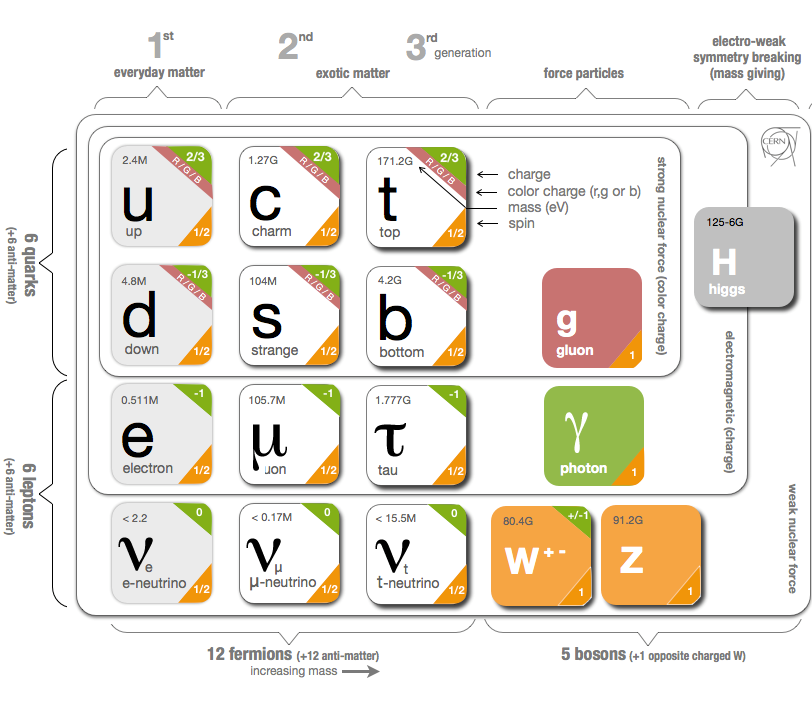
\includegraphics[width=0.90\textwidth]{../figs/Intro/StandardModel.png}}
    \caption{Standard Model Particles and Interations}
    \label{fig:SMtable}
  \end{center}
\end{figure}





